\documentclass[mscthesis]{usiinfthesis}
\usepackage{lipsum}
\usepackage{xcolor}

\usepackage{listings}

\lstdefinelanguage{algebra}
{morekeywords={import,sort,constructors,observers,transformers,axioms,if,
else,end},
sensitive=false,
morecomment=[l]{//s},
}



\title{Design and implementation of a firewall device} %compulsory
\mastermajor{Financial Technology and Computing}%optional
\specialization{main track}
%\subtitle{Subtitle: Reinventing the World} %optional 
\author{Bin Yong} %compulsory
\begin{committee}
\advisor{Prof.}{Student's}{Advisor} %compulsory
\coadvisor{Prof.}{Student's}{Co-Advisor}{} %optional
\end{committee}
\Day{Yesterday} %compulsory
\Month{September} %compulsory
\Year{2023} %compulsory, put only the year
\place{Lugano} %compulsory

%\dedication{To my beloved} %optional
%\openepigraph{Someone said \dots}{Someone} %optional

%\makeindex %optional, also comment out \theindex at the end

\begin{document}

\maketitle %generates the titlepage, this is FIXED

\frontmatter %generates the frontmatter, this is FIXED

\begin{abstract}
  \paragraph{}
  Design and implementation of a firewall device based on Raspberry Pi. The firewall will monitor and encrypt network activities. It is designed for someone who would like to sacrifice some compatibility to pursue better security but still wants some balance between security and convenience. A sensitive target, like an investigative journalist, could be a potential user of this device.

\end{abstract}

\begin{acknowledgements}
  \paragraph{}
  This document is a draft version of a working thesis of Bin Yong.
\end{acknowledgements}

\tableofcontents
\listoffigures %optional
\listoftables %optional

\mainmatter

\chapter{Introduction}
\paragraph{}
The goal of this work is to increase the chance of survival of the user from hacking, evasdropping, and digital fingerprinting. The device will work as a strict firewall which limits network activities and will also apply encryption standards to increase the difficulty of eavesdropping, and also to reduce the attack surface of fingerprinting. The device will run a TLS proxy to harden TLS protocol. It will use a screen to display selected real-time internet activities.
\paragraph{}
Using a hardware as a firewall has several advantages. Firstly, hardware
firewall can provide complete isolation between highly unsafe code,
like a browser, and firewall software (fun fact: I was hacked repeatedly
through personally harddened latest version of firefox while writing this
thesis). This could also work as a mitigation of CPU/BIOS level threats:
Firmware malwares, bootkits, and doubtable proprietray technologies like
Intel ME and the AMD PSP. Second, it will also provide convenience to the
user: the configuration of this portable device will be applied to protect
everything behind it, so people do not need to do the time consuming
configuration work on different softwares and operating systems one by one.
\paragraph{}
Even things that could not be configured will be under the restriction of the firewall. In example, people cannot untrust a built-in trusted root certificate from iPhone via Settings app.

\section{Existing commercial hardwares}
\paragraph{}
Commercial firewalls are expensive. In switzerland, the price of a entry
level firewall is more than twice of a raspberry pi. Raspberry Pi being
used in this work could be replaced with some cheaper alternatives, making
the cost will be even lower. Commercial firewalls also do not provide a
screen to display network activities in real-time.

\chapter{Operating system}

\paragraph{}
Due to its security-focused nature, OpenBSD would be a great choice when buiding a firewall. However, as a portable device, it is designed to work as a USB network device but OpenBSD does not contain a device mode in its USB stack. Linux provides USB gadget mode. Using the combination of ECM and RNDIS mode, most of Linux, Windows, BSD and MacOS could be supported. FreeBSD USB stack can run in device mode and provided 3 virtual network iterface templates but none of them works with Microsoft Windows\citep{freebsdhb:usb}. Considering the large market share of Microsoft Windows, linux is decided as the base OS of this firewall device.

\chapter{Packet filtering and forwarding}
\section{Design}
\paragraph{}
As the general principles, all traffics passed thorugh should be checked to against evasdropping. A plaintext connection should be channeled through strong encryptions or be discarded if unable to ensure its integrity.
\paragraph{}
A modern browser can satisify most of needs to interact with internet for working. So, allowing HTTP and HTTPS connections could make most of works done when facing a hostile network environment. Thus, everyting unnecessray to make this done are blocked. The firewall rules should be carefully made to filter out as much as possible and as early as possible, because everything on all layers of the Open Systems Interconnection model (OSI model) is protentialy vulnerable and the less network traffic being passed to the following components, the less chance a vulnerability can affect the firewall.
\paragraph{}
Proxies should be used to forward network traffics. There are advantages of using a proxy than forwarding packets like a router. First, a proxy can run under user level while packets forwarding run at kernel level. When there is a vulnerability, a userland one naturally to be less harmful than a kernel one. Second, proxies are easier and also safer to configure. It's hard to configure operatng system firewalls well. When the rules are not strict enough unexpected things may happen. In example, allowing any connection to 127.0.0.1 to success without a log, could cause potential problems if a malicious dhcp server assigned the address 127.0.0.1 to a physical network interface. Also, simply filtering packets by port numbers, addresses, and interfaces could not guarantee the packets being forwarded to the remote actually used by the protocols we are expecting. An attacker can simply let the receiving end of a reverse shell listen to an allowed port to bypass this kind of defense. By contrast, a proxy only works for the protocols that it can understand. when you are configuring a DNS proxy, the chance that your misconfiguration makes an attacker able to make http request over this proxy is very rare. They have to hack the firewall or create tunnels over those protocols to make their reverse shell work, which increased the difficulty of their operations. Third, the packets from the proxy will be encoded again by Linux network stack so the fingerprinting techniques that targeting TCP ad IP properties will useless to the devices under its protection.

\section{Implementation}
\paragraph{}
Nftables is integrated in modern linux systems. It can classify and filter network traffics. The firewall uses it to filter network packets. UDP 67 or 68 port and ARP packets are allowed for assigning IP addresses. UDP 53 is allowed from users to the firewall device for DNS requests, TCP 80, and TCP 443 are allowed for HTTP and HTTPS traffics. All other packets are filtered as early as possible.
\paragraph{}
Different proxies and RPC services are created to check connections, to forward traffcs, and to apply encryptions. Details are included in the chapters of the corresponding protocol.

\chapter{Dynamic Host Configuration Protocol (DHCP)}

\section{Introduction}
\paragraph{}
DHCP is widely used to dynamically assign a ip address to a new device connected to a network.

\subsection{The issue}
\paragraph{}
A client can expose its host name to the network from the 'client identifier' option or 'sname' field in the protocol. When in the same local network, the host name exposed by the DHCP protocol and other protocols can be used to locate the devices of the victim. If the name of a computer is straightforward enough, like "Yongbin's MacBoook Pro", the network administrator will be able to know the name of the owner of the computer from the first glance. The hardware address exposed to the network can also expose more information than just the address. Hardware address or Media Access Control (MAC) address can be used to reversly lookup the manufacturer and the manufacturer can help identify the owner. In example, the network administrator may lookup the MAC address of the a device to find out the manufacturer is company A and if the company A only sell its products in Country B and if C is the only person come from Country B then the chance that the device belongs to C would be high.

\section{Design}
\paragraph{}
Firewall should randomize both host name and MAC address. The randomized computer name should look normal to prevent being identified by potential attackers.

\lstdefinelanguage{conf}{
basicstyle=\ttfamily\small,
columns=fullflexible,
morecomment=[s][\color{purple}\bfseries]{[}{]},
morecomment=[l]{\#},
commentstyle=\color{gray}\ttfamily,
morekeywords={},
otherkeywords={=},
keywordstyle={\color{green}\bfseries}
}

\section{Implementation}
\paragraph{}
NetworkManager is used to manage physical connections of the firewall. By adding 'ethernet.cloned-mac-address=random' and 'wifi.cloned-mac-address=random' to the 'connection' section of NetworkManager.conf, the MAC address randomization will be done by NetworkManager. The 'ifconfig interface link random' command can also randomize the MAC address of a interface manually.
\paragraph{}
Host names of the firewall device is random generated while starting the system. The relevant code is inside rc.local. The name is crafted to look normal. The pattern of default computer name of Microsoft Windows and common names like iPad are used. Since the implementation of the client of the protocol could also be vulnerable, the combination of AppArmor and dhclient to mitigate this problem.
\paragraph{}
Dnsmasq is used to assign IP address of the users of the firewall it will also tell the devices behind the firewall to use the firewall as the DNS resolver.

\chapter{Domain Name System (DNS)}

\section{Introduction}
DNS is a protocol that translates the human readable domain names to the ip addresses of the remote server. The default configuration of many devices are to use plaintexts to do requests, which could easily be monitored by simply recording the packets and be attacked by methods like DNS spoofing.

\section{Design}
\paragraph{}
From the network administrator's view, all DNS queries sent out from firewall shoul be encrypted. From the user's view, nothing should be specially configured.

\section{Implementation}
\subsection{Outgoing requests}
\paragraph{}
A name resoving service is created to resolve domain name queries from firewall serices. It is a local RPC service that resolve domain name queries via public DNS-over-HTTPS (DoH) services. DoH can mitigate both passive surveillance and DNS spoofing attacks\citep{rfc:doh8}. DoT (DNS-over-TLS) is another DNS encryption standard that can do almost the same as DoH. The reason why use DoH instead of DoT is that DoT uses a unique server port number, 853, that can be easily filtered and identified as an encrypted DNS connection, while DoH, with the help of using the same port number and protocol as HTTPS, makes it much harder to be identified and filtered than DoT.
\subsection{Inside firewall}
\paragraph{}
A dnsmasq is started locally to resolve everything to localhost to make the firewall proxy to be applied as system-wide.
\subsection{Incoming requests}
\paragraph{}
A dnsmasq is started to resolve everything to the firewall device to make the firewall proxy to be applied to devices behind it.

\chapter{Transport Layer Security (TLS)}

\section{Management of certificates}

\subsection{Introduction}
All modern major operating systems managed a collection of trused certificates issued by certificate authorities (CAs) they choose. Those certificates are used to prove the validity of a public key. When makeing a TLS connection, local applications will check the path of the certificate provided by remote with local trusted collection to ensure secure connections.
\subsubsection{The issue}
\paragraph{}
Almost all TLS clients do not alert its user when the remote website presented a different certificate, which gives CAs the power to do man in the middle (MITM) attacks. Even if  do not want to do evil, their private key could still have been stolen. Thus, none of them are strictly trustworthy. However, whole TLS is based on it, if we trust none of those authorities, there will be almost no website we can use and things will be worse if without TLS.
\subsubsection{Exsting solutions}
\paragraph{}
SSL-pinning can prevent MITM attacks from a trusted CA when the user know the remote endpoint should use the certificate from another authority. However, configuring SSL-pinning to all the enspoints is hard and time consuming to average users and without a basic trusted environment, it will be unable to certain whether the configuration has done correctly. Even if the configuration is correct, it is still not strange for an enspoint to switch to another CA. Thus, to a firewall, this technique cannot be used as a general solution of the issue that can be applied to all endpoints.
\paragraph{}
Removing suspecious CAs from the trusted list could protect people from MITM attacks initiated by those CA. However, some systems and devices do proide the function of untrusting a CA. In example, iPhone needs a computer to enable such configuration and most of Android variants.
\subsection{Design}
\paragraph{}
The firewall should trust only the CAs that are being widely used in the internet. People should be able to further decide which certificates to trust. One can consider untrust following when making such decisios: the CAs of the place you are staying, the CAs of the place you come from, and their enemies and allies.
\subsection{Implementation}
\paragraph{}
Since SSL-pinning can only be used on a small number of enspoints to an andvanced user who can clearly know what is this meant to be, it is not implemented now. Manually management of the certificate can be done by Linux commands. The certificate of all outgoing TLS connection remote points are checked by TLS proxy.

\section{Proxy}
\subsubsection{Man in the mddle(MITM) attack}
\paragraph{}
Despite using MITM attack to insepect or protect encrypted connections has been used in firewalls and proxies for many years \citep{fortigate:deepinspection}, the tls proxy used in this firewall should not implement the same functioality. The reason is that when the firewall itself is compromised, the ability to decrypt TLS sessions will cause a disasteer to the devices behind it: the attacker will be able to easily modify the encrypted data transfered over a MITM proxy while the devices behind the firewall will alert nothing about the modification. However, if the firewall could not do MITM attack at all, the compromised still unable to see and modify encryptions, because the certificate verification of the devices behind this firewall is still working.
\subsubsection{Filtering certificates}
\paragraph{}
The key\_share extension sometimes makes the certificate invisible to the proxy. Thus, in order to filter certificates, the proxy will handshake with remote server with a sepearate connection to verify the certificate used by the remote host. A cache of trusted endpoints is used to reduce delay caused by certificate check connections
\subsubsection{Checking connections}
\paragraph{}
The proxy should parse handshake packets. It should check algorithms provided by ClientHello and ServerHello, to ensure strong encryption. Strenghten the connection by modifing handshake packets without MITM is not possible because the HMAC of all handshake packets is used for encryption.
\subsubsection{Implementation}
\paragraph{}
Since TLS proxy in charge of processing and forwarding the majority traffic of the firewall, c++ is used to develop the proxy due to its high performance capability. Upon receiving ClientHello from a client, the proxy checks the cryptography algorithms provided in it, like ciphersuites, and apply the best practices provided in rfc9325. The proxy extracts the Server Name Indication (SNI) from ClientHello to dertermine the actual destination of the request. Then use A RPC call to name service to resolve domain names. Then a TLS connection will be established to all of the addresses returned from the name service to selet the endpoints that is able to make a strong enough connection with a trusted certificate. The packets will be forwarded to one of the selected endpoints. Upon receiving the response ServerHello to the client, the proxy will check again whether the negotiation result comply to the best practce provided in rfc9325 and discard the connections that are not.


\chapter{Plaintext connections}

\section{HTTP}
\subsection{Implementation}
\paragraph{}
A proxy is created to filter and protect HTTP plaintext connections. The proxy check the host name with a known list of OCSP (Online Certificate Status Protocol) and CRL (Certificate Revocatoin List) servers. Only the connections to those servers are allowed to be plaintext because those connections usually to be OCSP over HTTP connections, which have no reason to be protected


\chapter{Date time synchornization}
\section{Introduction}
\paragraph{}
A correct time is required for TLS protocol to check certificates. Network Time Protocol (NTP) is used by most of modern systems to synchornize the clock with a remote server.
\subsection{The issue}
\paragraph{}
A problem of using a hardware like a Raspberry Pi is that it does not have a battery to keep the clock ticking after the power source is cut. So a time synchornization mechanism is a must for this firewall.
\paragraph{}
Many of operating systems are pre-configured to use a NTP server which having a unique domain name that can be used by a network administrator to identify the operating systems being used by the client.
\paragraph{}
Both the unique port number (UDP 123) and the unique domain names (time.windows.com, time.apple.com, and ubuntu.pool.ntp.org) makes NTP a protocol that can be easily identified and targeted. Various attacks can be done to the protocol itself\citep{ntp:attack}. The different in NTP behavior between different operatiing systems has been used in OS fingerprinting and tethering detection {osandtether}. Not to mention that the operating system being exposed by the domain name can also help an attacker to target the NTP client being used by the device.

\section{Design}
\paragraph{}
Give up on NTP, use HTTP/HTTPS instead. Use the "Date" header from the response of a HTTP server to synchornize date time in an acceptable accuracy. Usually, in order to hide, the attacks targeted to HTTP/HTTPS protocol do not want to make mistakes in the header of its attack vector.It's hard to say whether this request is made for time synchornization.

\section{Implementation}
\paragraph{}
Since TLS needs time to be correct to validate certificates, a plaintext HTTP request is made to do an initial synchornization. After the first step, the system clock is considered to be correct enought for making a TLS connection. So the second step is to extract date time from the header of a HTTPS response.

\chapter{Behavioral simulation}
\section{Introduction}
\paragraph{}
In previous chapters, the fact that network activities can be used to detect the user has been proved in different protocols. However, the efforts to reduce the leak of the information on those protocols are not enought when facing a more sophisticated network analyzation. In example, the connections to Windows update servers and App Store servers can be used to detect Windows and Apple devices citep{osandtether}, but the firewall has no reason to stop those connections. Even if the firewall blocked all OS specific connections, the domain leaked from TLS handshakes can also tell the evasdroppers what websites a person is watching and then may infer what the person is doing. Thus, the leak of the information seems to be inevitable.

\section{Design}
\paragraph{}
A service to simuluate different network activities is designed to solve ths issue. The goal is to hide user network activities inside the flood of fake network activities to increase the difficulty of an analyzer to produce useful reports. However, the risk of using this service is to produce a false alarm immediately and make the user blocked for tethering, make the user fired for browsering unrelated websites, etc.. To avoid the firewall to be compromised from browser vulnerabilities, browser-based simulation tools, like puppeteer, should not be used for implementation. It should also make plaintext traffics to attaract attentions from attackers and evasdroppers to make them less focused on the actual user traffics.

\section{Implementation}
\paragraph{}
The service is implemented in a python script named hood-actor.py. It can
\paragraph{}
\begin{figure}
  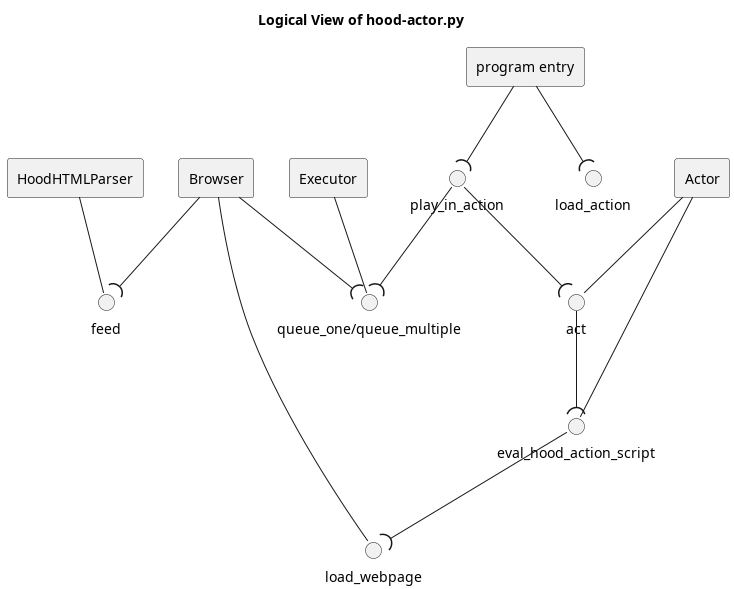
\includegraphics[width=0.9\textwidth]{graphics/puml/actor.png}
  \caption{Logic view of hood-actor.py}
  \label{fig:actor-logic-view}
\end{figure}

\chapter{Conclusions}

\section{Possible improvements for future}
\subsection{LSM and seccomp}
\paragraph{}
Use LSMs, like AppArmor, and seccomp to protect all as much process as possible. The programs that do not support seccomp can be changed by LD\_LOAD\_LIBRARY.

\subsection{Compile time hardening}
\paragraph{}
Use strict compiler options to harden everything, including kernel, like what Gentoo Linux is doing now, to try to mitigate some unpublished vulnerabilities, and also to increase the difficulty of attacking the firewall itself.

\subsection{Network stack fingerprinting}
\paragraph{}
Spoof network stacks, like TCP stacks and TLS stacks, to make the firewall and the devices behind it to be less detectable.

\subsection{Further use to libcomposite}
\paragraph{}
Libcomposite has the ability to make the device to show multiple roles to a host (a computer), which means the device can at the same time work as a USB mass storage device or as a USB CDROM, both of which can be used as a media of a Live DVD. Then the comptuer will be able to boot a live system from it. For a computer that password protected to boot from USB, we can also use this small device as a PXE server to make that computer boot from the network of the USB device.

\chapter{The attacks that I have encountered during the time I was working on this thesis}

\section{Malicious hardwares}
\paragraph{}
Normal attackers will use network, bluetooth or wifi for communications between malware and the host. In example, casting the screen to another device via wifi or sending keyboard inputs via bluetooth. Those kind of attacks can be detected by a RF detector. RF sheilding fabrc, RF detectors, and signal jammers could be used to fight against such kind of attacks.
\paragraph{}
However, There are still other ways exist. Some even without wireless communications. Despite I have already bought a RF detector to alert me wireless communications between unknown hardwares, unknown attackers still managed to monitor my progress by modified hardwares. Take the devices that I am using to develop this project for example. Raspberry 4B has a usb chip that can communicate to the power source. If the charger is specially crafted with the ability to forward the usb connection to the remote endpoint via power lines, then, with the help from the malware installed on the pi itself, data can be leaked silently via power lines even without any network connections to the computer. The same story can also be happened to the portable screen that I am using now. I have found two counter measurements to this kind of attack: One is to use USB-C to DC adapter when connecting a USB-C charger to the laptop. Another is to tape the two pins in the middle of male USB-A port to prevent data communications.

\section{Sounds}

\paragraph{}
Another attack that can bypass a rfkilled computer is to use AI / ML to identify the sounds of keyboard hits. The detected types can be send to remote via power lines or mobile phones. The sound could even be recorded from the room of a neighbor which makes this attack more stealthy than other methods. I use cardboards to extend the pillar of the key cap to shorten the key travel to lower the volume of the sound of the key hit to counter this attack but I am uncertain about the effect because I have no attack tools to test this. AliPay also used to use sound waves to transmit data between phones and vending machines. My raspberry pi recently started to emit strange noises from the speakers on the screen, which could because of the same technology being used for hackers.

\chapter[Short title]{A chapter title which will run over two lines --- it's for
  testing purpose}

\section{The first section}

\section{The second, math section}

\textbf{Theorem 1 (Residue Theorem).}
Let $f$ be analytic in the region $G$ except for the isolated singularities $a_1,a_2,\ldots,a_m$. If $\gamma$ is a closed rectifiable curve in $G$ which does not pass through any of the points $a_k$ and if $\gamma\approx 0$ in $G$ then
\[
  \frac{1}{2\pi i}\int_\gamma f = \sum_{k=1}^m n(\gamma;a_k) \text{Res}(f;a_k).
\]
\textbf{Theorem 2 (Maximum Modulus).}
\emph{Let $G$ be a bounded open set in $\mathbb{C}$ and suppose that $f$ is a continuous function on $G^-$ which is analytic in $G$. Then}
\[
  \max\{|f(z)|:z\in G^-\}=\max \{|f(z)|:z\in \partial G \}.
\]

\section[third]{A very very long section, titled ``The third section'', with
  a rather  short text alternative (third)}

\texttt{Some Test}
\lstset{language=algebra,linewidth=0.95\linewidth,breaklines=true,numbers=left,
  basicstyle=\ttfamily,numberstyle=\tiny,escapeinside={//*}{\^^M},
  mathescape=true}
\begin{lstlisting}
import IntSpec, ItemSpec;

sort cart; //*\label{sort}

constructors //*\label{begin-sig}
create() $\longrightarrow$ cart;
insert(cart, item) $\longrightarrow$ cart;
observers
amount(cart) $\longrightarrow$ int;
transformers
delete(cart, item) $\longrightarrow$ cart; //*\label{end-sig}

axioms //*\label{begin-axioms}
forall c: cart, i, j: item 

amount(create()) $=$ 0; //*\label{begin-amount}
amount(insert(c,i)) $=$ amount(c) $+$ price(i); //*\label{end-amount}
delete(create(),i) $=$ create(); //*\label{begin-delete}
delete(insert(c,i),j) $=$
if (i =$\:$= j) c
else insert(delete(c,j),i); //*\label{end-axioms}
end
\end{lstlisting}

As you can easily see from the above listing \citet{bbggs:iet07}
define something weird based on the BPEL specification
\citep{bpelspec}.
\nocite{*}

\appendix %optional, use only if you have an appendix

\chapter{Some retarded material}
\section{It's over\dots}

\backmatter

\chapter{Glossary} %optional

%\bibliographystyle{alpha}
%\bibliographystyle{dcu}
\bibliographystyle{plainnat}
\bibliography{biblio}

%\cleardoublepage
%\theindex %optional, use only if you have an index, must use
%\makeindex in the preamble
%\lipsum
1
\end{document}
\grid
